% Created 2016-10-08 sáb 07:34
\documentclass[11pt]{article}
\usepackage[utf8]{inputenc}
\usepackage[T1]{fontenc}
\usepackage{fixltx2e}
\usepackage{graphicx}
\usepackage{longtable}
\usepackage{float}
\usepackage{wrapfig}
\usepackage{rotating}
\usepackage[normalem]{ulem}
\usepackage{amsmath}
\usepackage{textcomp}
\usepackage{marvosym}
\usepackage{wasysym}
\usepackage{amssymb}
\usepackage{hyperref}
\tolerance=1000
\author{David Arroyo Menéndez}
\date{\today}
\title{Software LibrE y Economía}
\hypersetup{
  pdfkeywords={},
  pdfsubject={},
  pdfcreator={Emacs 24.4.1 (Org mode 8.2.10)}}
\begin{document}

\maketitle
\tableofcontents


\section{Abstract}
\label{sec-1}

En el presente artículo, se trata de establecer las relaciones entre
software libre y economía, para ello se establece un marco teórico en
el que se explican las raíces económicas de la cooperación aplicadas
en el contexto del software libre y un trabajo de análisis
cuantitativo que den vigor de realidad científica a ese marco. Para
este trabajo se ha elegido el caso de Linus Torvalds, con su comunidad
Linux y ver cómo se incrementa o no la ganancia en función de si él
coopera, o si coopera la comunidad.

\section{Marco Teórico}
\label{sec-2}

En (Mauss 2009: 70), se dice: "En la civilización escandinava y en
muchas otras, los intercambios y los contratos siempre se realizan en
forma de regalos, teóricamente voluntarios, pero, en realidad,
entregados y devueltos por obligación." El autor establece que en las
sociedades los regalos se dan y se reciben por norma social. Esto
tiene un valor explicativo en el mundo del software libre, pero a
nosotros nos interesa el juego económico. 

En el software libre se estable un juego cooperativo con dos
jugadores: el individuo y la comunidad. Dentro de los juegos
cooperativos, podemos ver interesantes dos posibles juegos para
explicar el comportamiento del software libre. Vamos a establecer la
hipótesis inicial de que el juego que se adapta bien es el juego de la
seguridad, en el que el equilibrio de Nash se encuentra en la
cooperación mutua

\begin{center}
\begin{tabular}{lll}
 & C & D\\
C & (3, 3) & (0, 2)\\
D & (2, 0) & (1, 1)\\
\end{tabular}
\end{center}


También debemos plantear que el problema a abordar es un problema de
acción colectiva esto es aquel en el que hay un bien común si todos ó casi
todos cooperan. La función de producción sería:

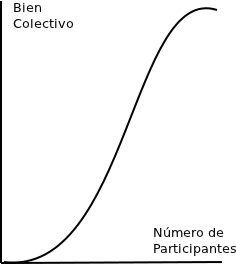
\includegraphics[width=.9\linewidth]{accion-colectiva.png}

Tal y como se ilustra en la gráfica cuando el número de participantes
es bajo el bien común ni siquiera se va a notar por lo que es
frustrante colaborar, si bien a partir de una cierta masa crítica las
posibilidades de alcanzar el bien común avanzan rápidamente y eso a su
vez anima a más participantes, sin embargo, una vez alcanzado no
importa mucho si suma más gente.

\section{Fuentes Documentales}
\label{sec-3}

\begin{itemize}
\item $\boxtimes$ Forbes: millonarios y empresas: \url{https://es.wikipedia.org/wiki/Anexo:Milmillonarios_seg\%C3\%BAn_Forbes#2000_Top_10}
\item $\boxtimes$ Estadísticas wikimedia: uso de sistemas operativos (año por año): \url{https://stats.wikimedia.org/wikimedia/squids/SquidReportOperatingSystems.htm}
\item $\square$ Participación de Linus Torvalds en Linux
\end{itemize}
% Emacs 24.4.1 (Org mode 8.2.10)
\end{document}
